
\section[Predicting things] {Supervising Machine Learning: Predicting things}






\subsection{You have done it before!}
\begin{frame}{You have done it before!}
	\begin{block}{Regression}<2->
		\begin{enumerate}
			\item<3-> Based on your data, you estimate some regression equation 	$y_i = \alpha + \beta_1 x_{i1} + \cdots + \beta_p x_{ip} + \varepsilon_i$
			\item<4-> Even if you have some \emph{new unseen data}, you can estimate your expected outcome $\hat{y}$!
			\item<5-> Example: You estimated a regression equation where $y$ is newspaper reading in days/week: $y = -.8 + .4 \times man + .08 \times age$
			\item<6-> You could now calculate $\hat{y}$ for a man of 20 years and a woman of 40 years -- \emph{even if no such person exists in your dataset}: \\
			$\hat{y}_{man20} = -.8 + .4 \times 1 + .08 \times 20 = 1.2$ \\
			$\hat{y}_{woman40} = -.8 + .4 \times 0 + .08 \times 40 = 2.4$
		\end{enumerate}
	\end{block}	
	
\end{frame}



\begin{frame}{}
	\huge{This is\\ Supervised Machine Learning!}
\end{frame}

\begin{frame}{\ldots but\ldots}
	\begin{itemize}
		\item<1-> We will only use \emph{half} {\tiny{(or another fraction)}} of our data to estimate the model, so that we can use the other half to check if our predictions match the manual coding (``labeled data'',``annotated data'' in SML-lingo)
		\begin{itemize}
			\item<2->e.g., 2000 labeled cases, 1000 for training, 1000 for testing --- if successful, run on 100,000 unlabeled cases
		\end{itemize}
		\item<3-> We use many more independent variables (``features'')
		\item<4-> For text analysis, IVs can be, e.g., word frequencies
	\end{itemize}
\end{frame}


\subsection{From regression to classification}
	
\begin{frame}[standout]
In the machine learning world, predicting some continous value is referred to as a \textcolor{orange}{regression} task. If we want to predict a binary or categorical variable, we call it a \textcolor{orange}{classification} task.

(quite confusingly, even if we use a logistic regression for the latter)
\end{frame}


\begin{frame}{Classification tasks}
For many computational approaches, we are actually not that interested in predicting a continous value. Typical questions include:
\begin{itemize}
	\item Is this article about topic A, B, C, D, or E?
	\item Is this review positive or negative?
	\item Does this text contain frame F?
	\item Is this satire? 
	\item Is this misinformation?
	\item Given past behavior, can I predict the next click?
\end{itemize}
\end{frame}



\begin{frame}[plain]
	\begin{columns}[]
		\column{.5\textwidth}
		
		{\tiny{http://commons.wikimedia.org/wiki/File:Precisionrecall.svg}}
		\makebox[\linewidth]{
			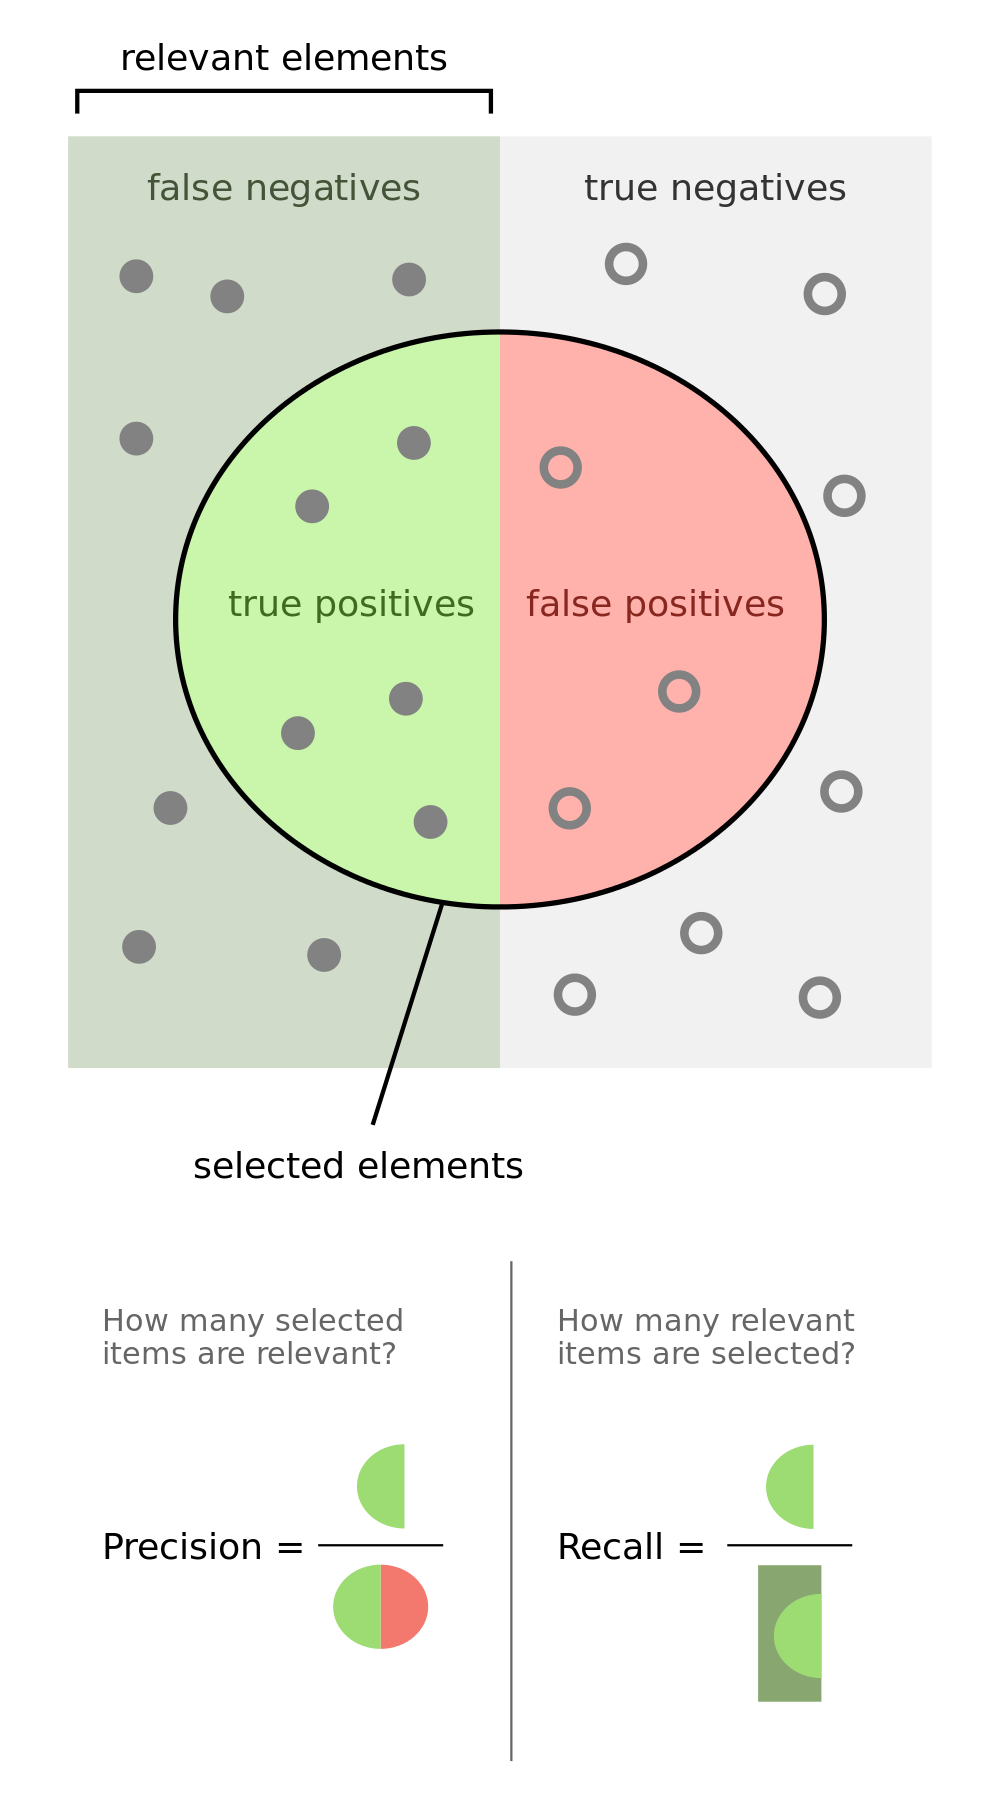
\includegraphics[width=\paperwidth,height=\paperheight,keepaspectratio]{precisionrecall.png}}
		
		\column{.5\textwidth}
		\begin{block}{Some measures}
			\begin{itemize}
				\item Accuracy
				\item Recall
				\item Precision
				\item $\text{F1}=2\cdot \frac{\text{precision}\cdot \text{recall}}{\text{precision}+\text{recall}}$
				\item AUC (Area under curve) $[0,1]$, $0.5=$ random guessing
			\end{itemize}
		\end{block}
		
		
	\end{columns}
	
\end{frame}





\begin{frame}{Different classification algorithms}

\begin{itemize}[<+->]
	\item It is an empirical question which one works best
	\item We typically try several ones and select the best
	\item (remember: we have a test dataset that we did \emph{not} use to train the model, so that we can assess how well it predicts the test labels based on the test features)
	\item To avoid $p$-hacking-like scenario's (which we call ``overfitting''), there are techniques available (cross-validation, later in this course)
\end{itemize}
\pause
To make it easier, we focus on binary classfication (``positive''/``negative''), but it doesn't really matter whether there are two or more labels)
\end{frame}






\begin{frame}{Naïve Bayes}
	\begin{block}{Bayes' theorem}
		$$ P(A \mid B) = \frac{P(B \mid A) \times P(A)}{P(B)} $$
	\end{block}
	\pause
	\textcolor{red}{A = Text is about sports\\
		B = Text contains `very', `close', `game'}.
	\pause
	Furthermore, we simply multiply the propabilities for the features:
	\textcolor{red}{$$P(B) = P(very\, close\, game) = P(very) \times P(close) \times P(game)$$}
	We can fill in all values by counting how many articles are about sports, and how often the words occur in these texts.
	\vspace{0.3cm}
	\tiny{
		(Fully elaborated example on \url{https://monkeylearn.com/blog/practical-explanation-naive-bayes-classifier/})}\\
\end{frame}

\begin{frame}{Naïve Bayes}
	\begin{itemize}[<+->]
		\item It's ``naïve'' because the features are treated as completely independent ($\neq$ ``controlling'' in regression analysis)
		\item It's fast and easy
		\item It's a good \emph{baseline} for binary classification problems
	\end{itemize}
\end{frame}




\begin{frame}{Na\"ive Bayes}
$$ P(\rm{label} \mid \rm{features}) =$$
$$ \frac{P(x_1 \mid label) \cdot P(x_2 \mid \rm{label})\ \cdot P(x_3 \mid label) \cdot P(label)}{P(x_1) \cdot P(x_2) \cdot P(x_3)}$$.

	
\begin{itemize}
	\item Formulas always look intimidating, but we only need to fill in how many documents containing feature $x_n$ have the label, how often the label occurs, and how often each feature occurs
	\item Also for computers, this is \emph{really easy and fast}
	\item Weird assumption: features are independent
	\item Often used as a baseline
\end{itemize}
\end{frame}




\begin{frame}{Logistic Regression}
	\begin{block}{Probability of a binary outcome in a regression model}
		$$p = \frac{1}{1 + e^{-(\beta_0 + \beta_1 x_1 + \beta_2 x_2 + \ldots + \beta_n x_n)}}$$
	\end{block}
	Just like in OLS regression, we have an intercept and regression coefficients. 
	We use a threshold (default: 0.5) and above, we assign the positive label (`good movie'), below, the negative label (`bad movie').
\end{frame}
\begin{frame}{Logistic Regression}
	\begin{itemize}[<+->]
		\item The features are \emph{not} independent.
		\item Computationally more expensive than Naïve Bayes
		\item We can get probabilities instead of just a label
		\item That allows us to say how sure we are for a specific case
		\item \ldots or to change the threshold to change our precision/recall-tradeoff
	\end{itemize}
\end{frame}

\begin{frame}{Support Vector Machines}
	\begin{columns}
		\column{.5\linewidth}
		\begin{itemize}
			\item	Idea: Find a hyperplane that best seperates your cases
			\item Can be linear, but does not have to be (depends on the so-called kernel you choose)
			\item Very popular 
		\end{itemize}
		\column{.5\linewidth}	
		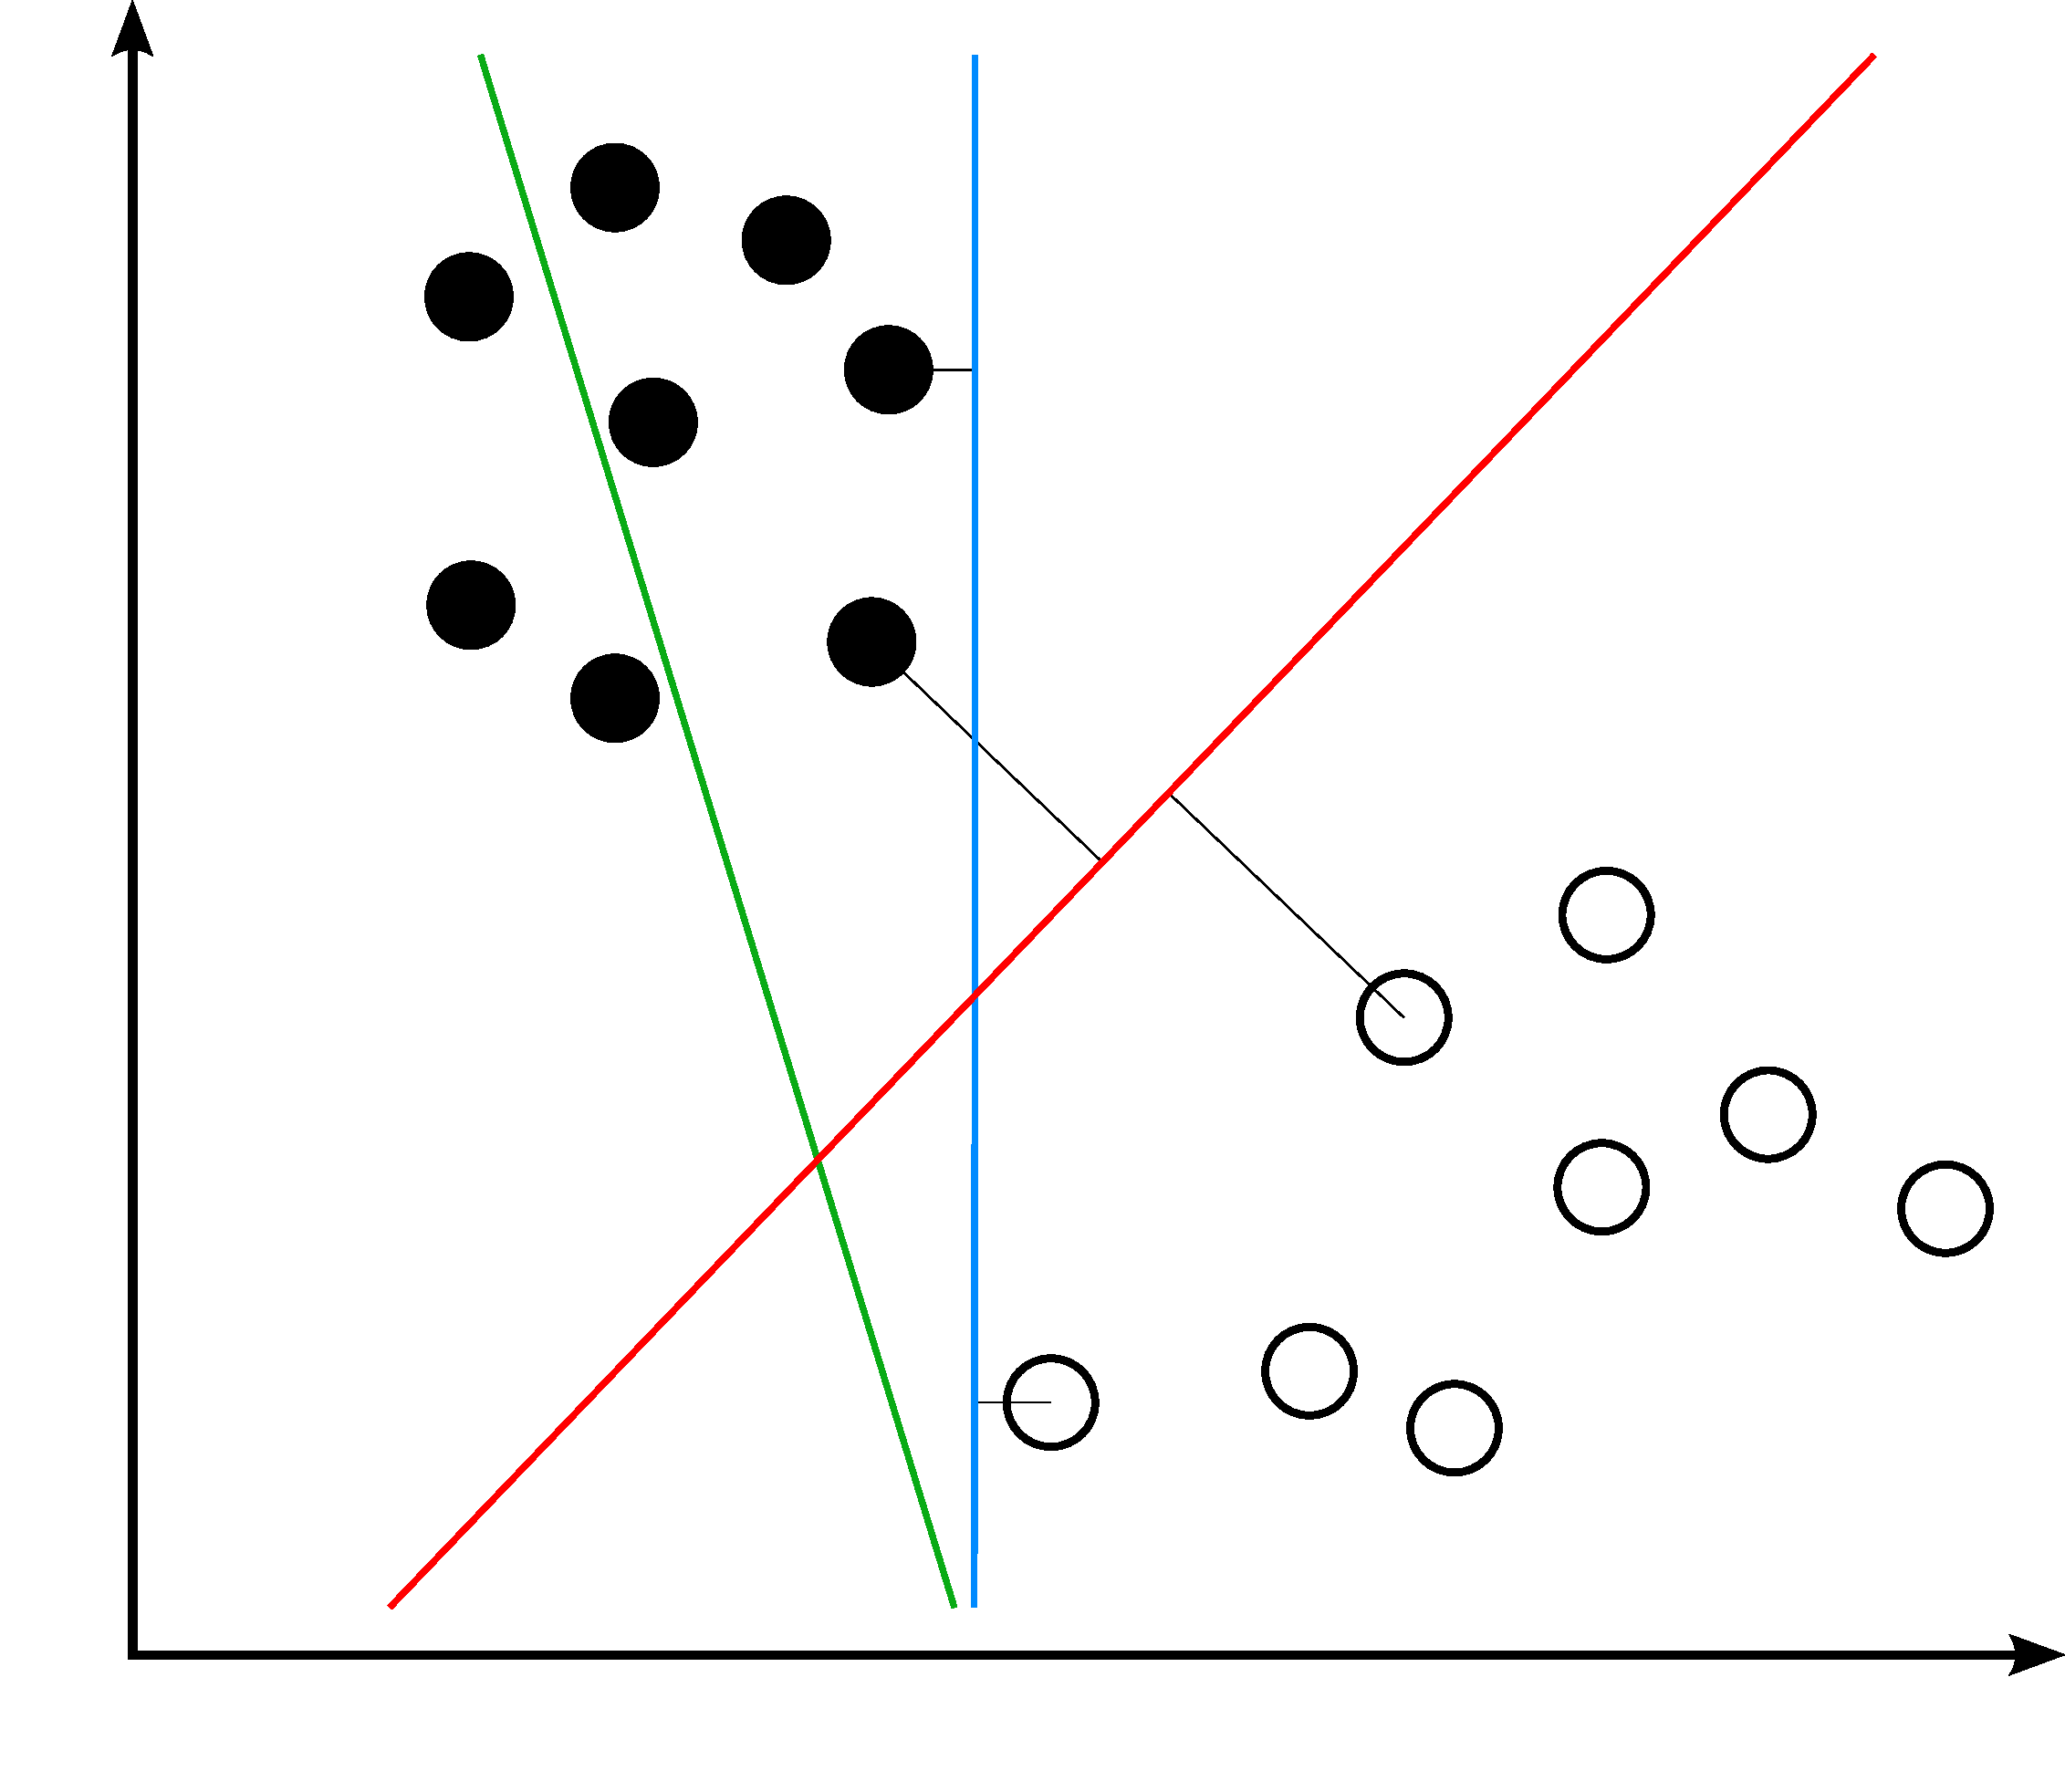
\includegraphics[width=.8\linewidth,height=.5\paperheight,keepaspectratio]{svm}
		\tiny{\url{https://upload.wikimedia.org/wikipedia/commons/b/b5/Svm\_separating\_hyperplanes\_\%28SVG\%29.svg}}
	\end{columns}
	\vfill
	\tiny{(Further reading: \url{https://monkeylearn.com/blog/introduction-to-support-vector-machines-svm/)}}\\
\end{frame}

\begin{frame}{SVM vs logistic regression}
\begin{itemize}
	\item for \emph{linearly separable} classes not much difference
	\item with the right hyperparameters, SVM is less sensitive to outliers
	\item biggest advantage: with the \emph{kernel trick}, data can be transformed that they \emph{become} linearily separable
\end{itemize}
\end{frame}


\begin{frame}{Decision Trees and Random Forests}
  \begin{columns}
    \column{.5\linewidth}
    \begin{itemize}[<+->]
    \item Model problem as a series of decisions (e.g., if cloudy then \ldots if temperature > 30 degrees then \ldots)
    \item Order and cutoff-points are determined by an algorithm
    \item Big advantage: Model non-linear relationships
    \item And: They are easy to interpret (!) (``white box'')
    \end{itemize}
    \column{.5\linewidth}	
		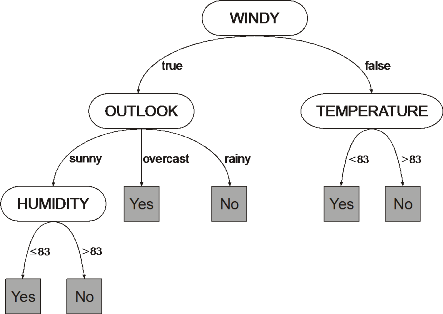
\includegraphics[width=.8\linewidth,height=.5\paperheight,keepaspectratio]{decisiontree}
		\tiny{\url{https://upload.wikimedia.org/wikipedia/en/4/4f/GEP\_decision\_tree\_with\_numeric\_and\_nominal\_attributes.png}}
	\end{columns}
\end{frame}
\begin{frame}{Decision Trees and Random Forests}
  \begin{block}{Disadvantages of decision trees}
    \begin{itemize}
    \item comparatively inaccurate
    \item once you are in the wrong branch, you cannot go `back up'
    \item prone to overfitting (e.g., outlier in training data may lead to completely different outcome)
    \end{itemize}
  \end{block}
  \pause
  Therfore, nowadays people use \emph{random forests}: Random forests \emph{combine} the predictions of \emph{multiple} trees
  $\Rightarrow$ might be a good choice for your non-linear classification problem
\end{frame}
